\section{基于Stacking的集成}
\label{sec:ensemble-stacking}

Bagging按固定规则聚合受到扰动的成员，Boosting则在逐轮训练中确定新成员的贡献。实际还可能已经有几种独立开发的模型。例如，同一房价任务中的线性模型概括整体趋势，近邻模型利用相似房屋的局部记录，森林表达特征交互。只挑一个模型会舍弃其他预测；一律等权平均又预先认定它们应当贡献相同。我们希望由数据学习怎样组合这些已有预测。

\term{Stacking}（stacked generalization，堆叠）把成员预测作为新特征，再训练一个组合模型。基学习器产生一级预测，\term{元学习器}（meta-learner）根据这些预测估计最终输出。元学习器可以学习线性权重，也可以在受控的函数类中学习非线性组合；是否能得到收益，取决于成员的样本外预测是否提供了互补信息\scite{wolpert1992stacked,breiman1996stacked}。

\subsection{Stacking}
\label{sec:ensemble-stacking-model}

\subsubsection{模型结构}

Stacking由基成员和元学习器两层组成，预测函数为
\[
 H(\bm x)=g_{\bm\theta}\!\left(h_1(\bm x),\ldots,h_M(\bm x)\right).
\]
其中$h_m$负责提取各自的预测信息，$g_{\bm\theta}$学习组合关系。基成员先对同一输入产生预测，元学习器把这些预测作为特征，输出最终结果。成员可以属于不同模型族；组合能够表达哪些关系，取决于元学习器允许的函数形式。

\subsubsection{参数学习}

\paragraph{生成折外训练特征}

设第$m$个成员模型为$h_m$。最直接的想法是：先在完整训练集上训练好每个成员，再把它们对训练样本的预测$h_m(\bm{x}_i)$当作元特征，喂给元学习器去学组合权重。这样做有一个隐蔽而致命的陷阱。设想成员中有一个“死记硬背”的模型，比如$1$近邻：它对每条训练记录的预测就是这条记录自己的标签，训练集上的正确率是$100\%$。元学习器看到这样的元特征，自然会认定“这个成员永远对，全听它的”，于是把几乎全部权重给它。可一到新样本，$1$近邻的表现可能远不如其他成员，元学习器学到的组合也就完全不可靠。问题的根源是：成员在训练记录上的预测已经“偷看过”这些记录的答案，而部署时成员面对的是没见过答案的新输入，两种预测的可信度完全不同；元学习器必须在“成员没见过答案”的条件下学习，才能学到对新样本有效的组合。

怎样让每条训练记录都得到一份“成员没见过它答案”的预测？交叉验证给出了答案，Stacking据此生成\term{折外预测}（out-of-fold prediction, OOF prediction）。思路是“轮流留出”：把训练样本划分为$K$个互不相交的折$V_1,\ldots,V_K$，每次留出一折、用其余折训练成员，再让它去预测被留出的那一折；轮完$K$次，每条记录都恰好被一个“没用它训练过”的成员预测过一次。具体地，对每个成员类型$m$和每个折$k$，只用$D_n\setminus V_k$训练临时模型$h_m^{(-k)}$，再预测$V_k$中的样本。若样本$i$属于$V_{k(i)}$，元特征定义为
\begin{equation}
  z_{i,m}
  =
  h_m^{(-k(i))}(\bm{x}_i).
  \label{eq:ensemble-oof-feature}
\end{equation}
把所有成员的折外预测拼成$\bm{z}_i=(z_{i,1},\ldots,z_{i,M})^{\top}$，再由元学习算法$\mathcal{G}$训练
\[
  g=\mathcal{G}\!\left(\{(\bm{z}_i,y_i)\}_{i=1}^{n}\right).
\]
对每个样本，临时成员的拟合数据排除了它所在的折，其标签只在后续元学习器训练中使用。图\ref{fig:ensemble-stacking-oof}展示了折外矩阵的形成过程。

\begin{figure*}[htbp]
  \centering
  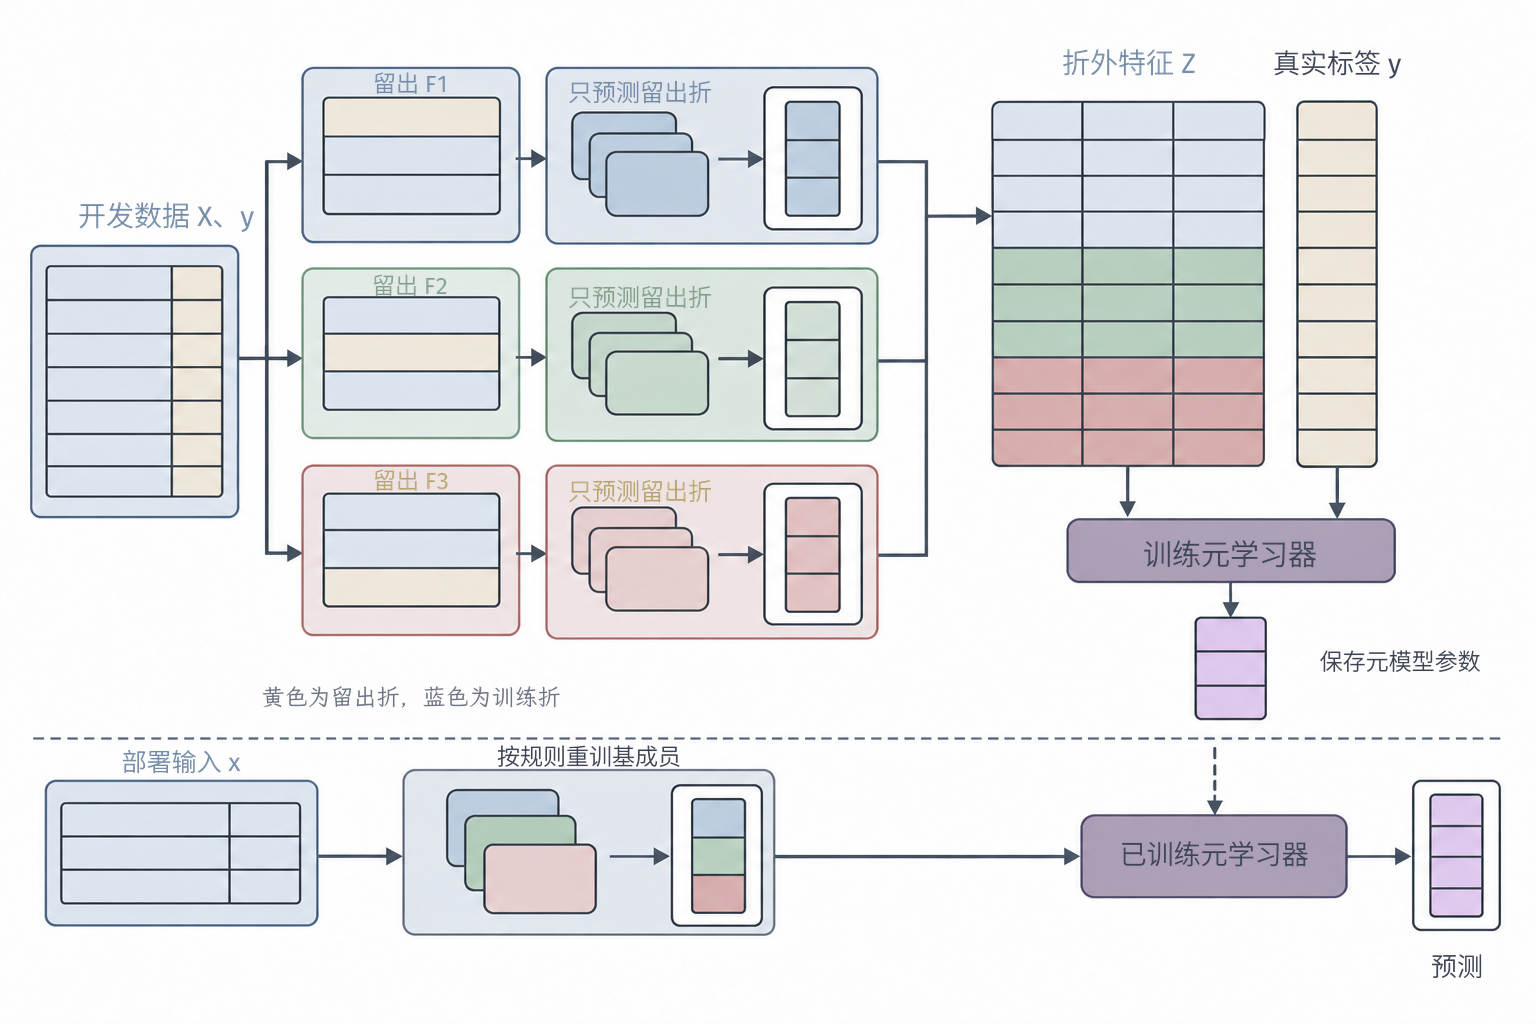
\includegraphics[width=130.048mm]{figures/04-classic-models/00-shared/generated/ensemble-stacking-oof/figure.png}
  \caption{三折Stacking的折外特征构造。每一折轮流作为留出折，临时成员只在其余两折训练，并为留出折产生预测；拼接三次预测得到完整折外矩阵$\bm{Z}$，元学习器以$\bm{Z}$为输入并使用对应标签拟合。部署阶段的基成员还需按预先规定的方式重训或保留。}
  \label{fig:ensemble-stacking-oof}
\end{figure*}

分类成员若输出$C$维概率向量，一个成员通常贡献$C$列元特征；二分类时也可以只保留一个类别概率。类别硬判断省去了得分中的排序或置信信息，不同成员的得分还可能采用不同尺度。元训练与部署使用一致的输出形式，正则化再控制尺度及相关预测对组合的影响。

\paragraph{确定部署成员}

折外矩阵用于训练元学习器，但部署时还需要能预测新输入的基成员。一种做法是在完整训练集上重新拟合每类基学习器$\widehat{h}_m$，预测
\[
  \widehat{y}
  =
  g\!\left(
    \widehat{h}_1(\bm{x}),\ldots,\widehat{h}_M(\bm{x})
  \right).
\]
全量重训利用全部开发数据，但训练规模增加可能改变预测分布，元学习器训练时只看过较小训练集产生的输出。也可保留各折成员，先平均它们对新输入的预测，再送入元学习器；这样沿用折内模型，同时增加了存储与推理次数。两方案的输入分布差异仍由完整验证检验。

部署方案确定后，需要评价基成员与元学习器共同形成的预测流程。基学习器的特征处理、类别编码和超参数搜索必须在相应训练折内完成。若先用全部数据选择特征或编码，再只把模型拟合放进交叉验证，信息仍可能从留出折进入元特征。

\subsubsection{多层组合与输入相关权重}

\paragraph{支持多层组合关系}
\label{sec:ensemble-stacking-multilevel}

若一层组合仍不足以描述成员间关系，可以把中间层输出继续送入下一层。令$\bm a_0(\bm x)=(h_1(\bm x),\ldots,h_M(\bm x))^{\top}$，多层结构写为
\[
 \bm a_\ell(\bm x)=g_{\ell,\bm\theta_\ell}(\bm a_{\ell-1}(\bm x)),
 \quad \ell=1,\ldots,L,
 \qquad H(\bm x)=\bm a_L(\bm x),
\]
其中最后一层维数与所需输出一致。也可把原始特征或较早层输出拼接到某层输入，但须明确拼接对象。训练第$\ell$层时，对每个留出折，都要在其余数据上重新拟合完整下层流程，再为该折产生$\bm a_{\ell-1}$。只让底层成员留出当前记录，而让中间组合层使用其标签，仍会泄漏。逐层增加表达能力的代价是重复拟合、更多参数与部署计算，需要用完整外层验证判断是否值得。

\paragraph{支持输入相关组合}
\label{sec:ensemble-stacking-input-dependent}

固定线性权重让所有输入使用同一组成员贡献。如果线性模型在稀疏区域更稳定、近邻模型在稠密区域更准确，可以让权重随输入改变。一种具体结构是用门控函数$b_m(\bm x;\bm\theta)$产生非负归一化权重：
\[
 w_m(\bm x;\bm\theta)
 =\frac{e^{b_m(\bm x;\bm\theta)}}{\sum_{j=1}^M e^{b_j(\bm x;\bm\theta)}},
 \qquad
 H(\bm x)=\sum_{m=1}^M w_m(\bm x;\bm\theta)h_m(\bm x).
\]
基成员固定后，用折外预测$z_{i,m}$估计门控参数：
\[
 \widehat{\bm\theta}\in\argmin_{\bm\theta}
 \sum_i\ell\!\left(y_i,\sum_m w_m(\bm x_i;\bm\theta)z_{i,m}\right)
 +\lambda\Omega(\bm\theta).
\]
门控输入也须按训练折预处理。部署时把折外预测替换为预定部署成员的输出；各类别概率可以用同一组权重逐类组合。这种加权仍计算全部参与成员，第\ref{sec:ensemble-dynamic-selection}节的动态选择则可进一步只调用一个成员或某个子集。

\subsection{Blending}
\label{sec:ensemble-blending}

\subsubsection{模型结构}

折外构造让每条训练记录都获得一份未使用自身标签的成员预测，却要为每种成员重复拟合多个折内模型。成员训练昂贵时，这个成本可能难以承担。\term{Blending}改用一次留出来构造元特征：把开发数据分为基训练集$D_{\mathrm{base}}$和组合训练集$D_{\mathrm{blend}}$，基成员只在前者拟合，再预测后者，元学习器用这些预测与对应标签训练。每种成员只需一次用于元特征的拟合，代价是两层不再都利用全部开发样本。

\subsubsection{参数学习}

训练数据由两层分用：基成员在$D_{\mathrm{base}}$拟合，元学习器只使用$D_{\mathrm{blend}}$的预测与标签。在开发数据总量固定时，组合训练集$D_{\mathrm{blend}}$占比较小，元学习器用于估计组合关系的记录较少，估计可能不稳定；$D_{\mathrm{blend}}$占比增大，留给基训练集$D_{\mathrm{base}}$的记录随之减少，基成员训练信息也会减少。多次随机划分并平均可以减小单次划分的偶然性，但它重新引入多次训练，已经不再具有单次Blending的全部成本优势。

部署时若把$D_{\mathrm{blend}}$加入基成员重新训练，基预测分布可能相对元学习器训练时发生变化；若不加入，则没有充分利用已有标签。重训方式因此属于模型配置，需要先确定，再用未参与选择的数据评价实际组合。

\Needspace{10\baselineskip}
\subsection{受约束线性Stacking}
\label{sec:ensemble-constrained-linear-stacking}

\subsubsection{模型结构}

成员预测往往高度相关。例如两棵森林只在少量输入上稍有差别，元学习器就可能用很大的正权重与负权重相互抵消，拟合这些细小差异；成员输出稍有变化，组合也会随之放大变化。若希望用较少参数组合，并限制这种抵消，可以把元学习器限制为$b+\bm w^{\top}\bm z$，其中$b$是截距，$\bm w$是成员权重，$\bm z$汇集成员预测。在截距为零且权重非负时，再把权重和限制为一，组合预测就落在成员预测的范围内。

\subsubsection{参数学习}

在回归折外矩阵$\bm{Z}\in\mathbb{R}^{n\times M}$上，可以通过带惩罚的经验目标估计截距与权重：
\begin{equation}
  (\widehat{b},\widehat{\bm{w}})
  \in
  \argmin_{b,\bm{w}}
  \frac{1}{n}
  \sum_{i=1}^{n}
  \ell\!\left(
    y_i,
    b+\bm{w}^{\top}\bm{z}_i
  \right)
  +\lambda\lVert\bm{w}\rVert_2^2.
  \label{eq:ensemble-linear-stacking}
\end{equation}
权重约束控制组合允许的尺度和方向。在$b=0$时，仅要求$w_m\geq0$得到非负线性组合，仍可能放大预测；仅要求$\sum_mw_m=1$得到仿射组合，仍可因负权重而外推。只有同时满足$b=0$、$w_m\geq0$和$\sum_mw_m=1$，才是成员预测的凸组合，输出必定位于成员预测的凸包内。非负约束排除了成员之间的正负抵消，归一化进一步限制整体尺度；有效校正若需要负权重或截距，约束会缩小候选类并增加逼近误差。

权重大小同时受输出尺度、成员相关性和损失函数影响。两个成员预测近乎相同，线性模型可以在它们之间任意分配相近作用；一个成员输出的数值范围更大，也会改变未标准化正则项下的权重。估计权重反映给定尺度、相关性与损失下的联合拟合，而非成员独立贡献。对同一类别集合上的概率向量，使用同一组满足上述凸组合条件的权重逐类组合，结果保持概率单纯形约束，样本外校准再检查概率与实际频率的对应。

\Needspace{10\baselineskip}
\subsection{Super Learner}
\label{sec:ensemble-super-learner}

\subsubsection{模型结构}

不同学习器各有合适的数据条件，事先往往难以指定最佳成员及权重。\term{Super Learner}把候选模型库、折外预测和损失最小化组织成完整程序：用同一套折外数据比较候选，再选择单个成员或学习受约束组合。回归中常用的组合结构为$H(\bm x)=\sum_m w_m h_m(\bm x)$，其中$w_m\geq0$且$\sum_mw_m=1$\scite{vanderlaan2007superlearner}。

\subsubsection{参数学习}

先按式\eqref{eq:ensemble-oof-feature}生成候选库的折外矩阵$\bm Z$。离散版本选择折外平均损失最小的一列；连续组合版本则求解
\[
 \widehat{\bm w}\in\argmin_{\bm w\in\Delta_M}
  \frac1n\sum_{i=1}^n\ell\!\left(y_i,\sum_{m=1}^M w_m z_{i,m}\right),
 \qquad
 \Delta_M=\{\bm w:w_m\geq0,\ \sum_mw_m=1\}.
\]
例如平方损失给出带单纯形约束的最小二乘问题。随后在全部开发数据上重训各基成员，保留已学权重用于组合。候选库也可以预先包含不同模型族和超参数设置，但每列的折外预测必须遵守相应训练范围。

这里的折外损失参与了权重选择，不能再充当整个Super Learner未经选择的最终测试结果。若要比较不同候选库、组合约束或完整Stacking程序，应在外层验证中重新完成内层训练与权重选择。Super Learner与受约束Stacking因此可以共享同一预测结构；前者强调候选库及交叉验证选择程序，后者强调组合层的形式。

\subsection{模型对比与总结}
\label{sec:ensemble-stacking-comparison}

这些方法改变的是组合训练的不同环节。Stacking与Blending分别采用折外预测与一次留出预测；受约束线性组合限制元学习器，多层结构增加组合深度，门控结构使权重依赖输入。Super Learner进一步把候选库和交叉验证损失规定为完整选择程序。表\ref{tab:ensemble-stacking-comparison}据此比较数据安排、组合方式及成本。

\begin{table*}[htbp]
  \centering
  \small
  \begin{tabularx}{\linewidth}{@{}>{\raggedright\arraybackslash}p{25mm}*{5}{>{\raggedright\arraybackslash}X}@{}}
    \toprule
    方法 & 元特征来源 & 数据利用 & 组合规则 & 主要成本 & 主要风险 \\
    \midrule
    Stacking & $K$折折外预测 & 每个样本都产生元特征 & 可线性或非线性 & 每类成员需多次折内拟合 & 折外流程不完整造成泄漏 \\
    Blending & 固定留出集预测 & 元学习器只用留出集 & 可线性或非线性 & 基成员用于元特征时只拟合一次 & 划分敏感与重训分布变化 \\
    受约束线性Stacking & 通常为折外预测 & 与所用划分一致 & 非负、和为一或正则化线性组合 & 组合层较轻量 & 约束可能排除有效校正 \\
    Super Learner & 交叉验证预测与风险 & 由交叉验证方案决定 & 在预定库和组合类中选择 & 候选库越大，训练与选择成本越高 & 候选库遗漏合适模型，或选择过程泄漏 \\
    \bottomrule
  \end{tabularx}
  \caption{Stacking及其代表性变体。表中“数据利用”描述元学习器训练阶段；部署前是否用完整开发数据重训基成员，还需作为流程的一部分单独规定。}
  \label{tab:ensemble-stacking-comparison}
\end{table*}

部署前的全量重训还会改变成员产生预测时所用的训练规模。选择保留折内成员还是重训成员，需要与组合层一起评价，不能只比较各基成员的单独测试结果。比较上述方法时，应固定输出语义、预处理范围和训练预算，再判断新增组合是否改善完整流程的预测。
